\documentclass[a4paper, 12 pt]{article}                                	%TIPO DE FOLHA, TAMANHO DA FONTE E CLASSE DO DOCUMENTO
\usepackage[utf8]{inputenc}                                            	%IDENTIFICAÇÃO DE CARACTERES
\usepackage{mathptmx}
\usepackage{amsmath}
\usepackage{graphicx}                                                  	%ANEXAR IMAGENS
\usepackage{float}
\usepackage{amssymb}
\usepackage{makeidx}
\usepackage{pdfpages} 													% ANEXAR PDF
\usepackage[hidelinks]{hyperref}										% MONTAR OS LINKS E ESCONDER A MARCANÇÃO DE LINKS DO SUMMÁRIO
\usepackage[toc,page]{appendix}                                        
\usepackage[brazil]{babel}                                             	% PACOTE PARA PORTUGÊS - BR
\usepackage{indentfirst}                                               	% AJUSTAR PRIMEIRA LINHA DO PARAGRÁFO
\usepackage[top=2cm, bottom=2cm, left=2.5cm, right=2.5cm]{geometry}    	% MARGENS 
\usepackage{setspace}                                                  	% UTILIZAÇÃO DE ESPAÇAMENTO

\setlength{\parindent}{1.5cm}                  							%AJUSTE DO PARAGRÁFO

\begin{document}
	%%%%%%%%%%% CAPA %%%%%%%%%%%
	\begin{titlepage}
		\begin{center}
			\begin{figure}
				\centering
				
\includegraphics[scale=2.5]{figuras/uece.png}
			\end{figure}
			
			\large
			\textbf{UNIVERSIDADE ESTADUAL DO CEARÁ - UECE\\ \vspace{0.5cm}
				FACULDADE DE FILOSOFIA DOM AURELIANO MATOS - FAFIDAM\\ \vspace{0.5cm}
				NOME DO CURSO \\ \vspace{0.5cm}
				DISCIPLINA: \\ \vspace{0.5cm}
				PROFESSOR(A): \\ \vspace{0.5cm}
				ALUNO(A):\textnormal{ FULANO DE TAL} \\ \vspace{5cm}
				RELATÓRIO DE ... \\ \vspace{7cm}
				Cidade - SIGLA ESTADO \\ \vspace{0.5cm} \today{}}  % "\today":  DATA (PREENCHIMENTO AUTOMÁTICO)
		\end{center}
	\end{titlepage}
		
	
	\newpage
	\begin{center}
		UNIVERSIDADE ESTADUAL DO CEARÁ - UECE\\ \vspace{0.5cm}
		FACULDADE DE FILOSOFIA DOM AURELIANO MATOS - FAFIDAM\\ \vspace{0.5cm}
		NOME DO CURSO \\ \vspace{0.5cm}
		ALUNO(A):\textnormal{ FULANO DE TAL} \\ \vspace{8cm}
		
		\begin{flushright}
			\hspace*{8cm}\parbox{8.5cm}{{Relatório apresentado ao curso de licenciatura plena em Física da Faculdade de Filosofia Dom Aureliano Matos da Universidade Estadual do Ceará, como parte da exigência da disciplina de Estágio de Ensino de Física 2 ministrada pela Professora Francisca Daniele Costa De Lima Beserra.}}
			
		\end{flushright}
		
		\vspace{8cm}
		\textbf{Cidade - ESTADO}
		
		\vspace{0.5cm}
		\today{}		% DATA (PREENCHIMENTO AUTOMÁTICO)
	\end{center}
	\thispagestyle{empty}
	
	\newpage 
	
	%%%%%%%%%% PÁGINA DE ASSINATURA %%%%%%%%%%%%%%%%
	\begin{center}
	UNIVERSIDADE ESTADUAL DO CEARÁ - UECE\\ \vspace{0.5cm}
	FACULDADE DE FILOSOFIA DOM AURELIANO MATOS - FAFIDAM\\ \vspace{0.5cm}
	NOME DO CURSO \\ \vspace{0.5cm}
	ALUNO(A):\textnormal{ FULANO DE TAL} \\ \vspace{5cm}
		
		\rule{15 cm}{0.008 cm}
		Aluno(a)
		
		\vspace{5 cm}
		
		\rule{15 cm}{0.008 cm}
		Coordenador(a) de Estágio: % NOME DO COORDENADOR DO ESTÁGIO
		
		\vspace{9 cm}
		\textbf{Cidade - ESTADO}
		
		\today{}			% DATA (PREENCHIMENTO AUTOMÁTICO)
		
	\end{center}
	\thispagestyle{empty}
	
	\newpage
	\tableofcontents                         %SUMÁRIO (PREENCHIMENTO AUTOMÁTICO)
	\thispagestyle{empty}
	
	
	\newpage                                 %NOVA PÁGINA
	
	\setstretch{1.5}                         %ESPAÇAMENTO
	
	
	%%%%%%%%%% ELEMENTOS TEXTUAIS %%%%%%%%%%%%%%%
	\section{Introdução}
	\label{sec:introducao}
	
	%%% EXEMPLO DE INTRODUÇÃO:
	O presente trabalho visa relatar o processo de estágio de física 2 vivenciado
	durante a disciplina de Estágio de Ensino de Física 2 na turma do 2º ano do Colégio Oliveira Paiva, ministrado pela Professora Fabiane Souza, do curso de Licenciatura plena em Física da Faculdade de Filosofia Dom Aureliano Matos.
	
	A Escolha do Colégio Oliveira Paiva, localizado em Morada Nova, foi devido a proximidade do Professor Matheus Soares, o que facilitou na fluidez da relação estagiário - supervisor. Então pedi ao mesmo, que dá aulas de física e matemática na referida escola a bastante tempo, para estagiar em seus horários. Muito bem acolhido pelo Professor e Coordenação, foi dado início ao estágio supervisionado.
	
	O estágio foi realizado seguindo uma turma de segundo ano no turno matutino do Colégio Oliveira Paiva. O presente relatório está dividido em encontros e possui apontamentos de elementos sobre as turmas, o professor, aulas, atividades e minha experiência em geral.
	
	\setstretch{1.5}
	\section{Objetivos}
	
	\begin{itemize}   %% EXEMPLO DE MONTAGEM DOS ITENS
		
		%%% EXEMPLO DE OBJETIVOS:
		\item Buscar vivenciar e aprender na prática o manejo de uma aula;
		\item Observar o comportamento da turma e identificar as possíveis práticas para correções dos problemas apontados;
	\end{itemize}
	
	
	\
	%\
	%\
	
	\setstretch{1.5}
	\section{Fundamentos Teóricos}
	
	\setstretch{1.5}
	
	MONTAR A FUNDAMENTAÇÃO TEÓRICA QUE DEFENDA O ENSINO DE CIÊNCIAS MOSTRANDO SUA IMPORTÂNCIA PARA A SOCIEDADE.
	
	
	\section{Metodologia}
	\label{sec:metodologia}
	
	INFORMAR A METODOLOGIA ABORDADA NO ESTÁGIO. DESCREVER A DIVISÃO DA EXPERIÊNCIA DETALHADAMENTE POR MOTIVO DE ORGANIZAÇÃO TEXTUAL.
	
	\subsection{1º encontro: CONTEÚDO ABORDADO} 2º ano - (horário de inicio e fim da aula) - (quantidade de aula : tempo de aula em minutos).
	
	DISCORRER SOBRE O PRIMEIRO ENCONTRO  
	
	
	\
	\setstretch{1.5}                        %ESPAÇAMENTO PRO RESTANTE DO TEXTO (NÃO RETIRAR!!!)
	\subsection{Atividades diversas}
	
	DISCORRER SOBRE ATIVIDADES DIVERSAS (A ESCOLHA DO LOCAL DA SUBSEÇÃO FICA A CARGO DO ESTAGIÁRIO)
	
	\
	\subsection{2º encontro: CONTEÚDO ABORDADO} 2º ano - (horário de inicio e fim da aula) - (quantidade de aula : tempo de aula em minutos).
	
	DISCORRER SOBRE O SEGUNDO ENCONTRO 
	
	OBS.: A ORGANIZAÇÃO DA ABORDAGEM METODOLÓGICA FICA A CRITÉRIO DO ESTAGIÁRIO
	
	\newpage
	\section{Caracterização do estágio}
	
	NESSE TÓPICO O ESTAGIÁRIO DEVE ESCREVER SOBRE:
	
	NOME DA ESCOLA, ENDEREÇO E CONTATO;
	
	INFORMAÇÕES SOBRE A TURMA;
	
	INFORMAÇÕES SOBRE A ESCOLA (DISPONÍVEL NO PROJETO POLÍTICO PEDAGÓGICO);
	
	INFORMAÇÕES A REPEITO DA LDB - Lei de Diretrizes e Bases da Educação Nacional
	
	\newpage
	\section{Discussão}
	
	NESSE TÓPICO O ESTAGIÁRIO DEVE MONTAR SUA DISCUSSÃO BASEADO EM SUA EXPERIÊNCIA DE ESTÁGIO, INFORMAR A IMPORTÂNCIA DA DISCIPLINA E EXPRESSAR CRÍTICAS CONSTRUTIVAS.
	
	
	\newpage
	\section{Conclusão}
	
	O ESTAGIÁRIO DEVE CONCLUIR, NESTE TÓPICO, A SERVENTIA DO ESTÁGIO EM SUA PASSAGEM NA LICENCIATURA E DESCREVER SUA AUTO-CRÍTICA, OS PONTOS QUE PODEM A SEREM MELHORADOS, PONTOS QUE FOI MODIFICADO AO LONGO DO PROCESSO, ETC.
	
	
	\newpage
	\section{Referências Bibliográficas}   
	
	EXEMPLOS DE CITAÇÃO:
	%%%%%%%%% DICA: PEGAR CITAÇÃO NO SITE DO GOOGLE ACADÊMICO (GOOGLE SCHOLAR) - BASTA ESCREVER O NOME DA OBRA %%%%%%%%%%
	
	
	CARVALHO, Ana Maria Pessoa de et al. Ciência no Ensino Fundamental: O conhecimento físico do mundo. São Paulo: Scipione, 2007;
	
	\
	
	NEWTON, Villas Boas; HELOU, Ricardo. Tópicos de física. 18a edição, São Paulo: Editora Saraiva 2007. V.2;
	
	\
	
	Sarup, Madan. ``Las perspectivas interaccionista y marxista en la sociología de la educación: una introducción." Marxismo y sociología de la educación. Akal, 1986.
	
	\newpage
	
	%%%%%%%%% APÊNDICE: INCLUSÃO DE DOCUMENTOS ELABORADOS PELO AUTOR QUE POSSAM COMPLEMENTAR O TEXTO %%%%%%%%%
	%%%%%%%%% ESPAÇO ONDE PODE SER INCLUÍDO FICHA DE OBSERVAÇÃO, PLANOS DE AULA, ETC %%%%%%%%%%%
	\appendix
	\section{Ficha de observação}  % EXEMPLO DE INCLUSÃO DE PDF  
	\label{ap:ficha}
	%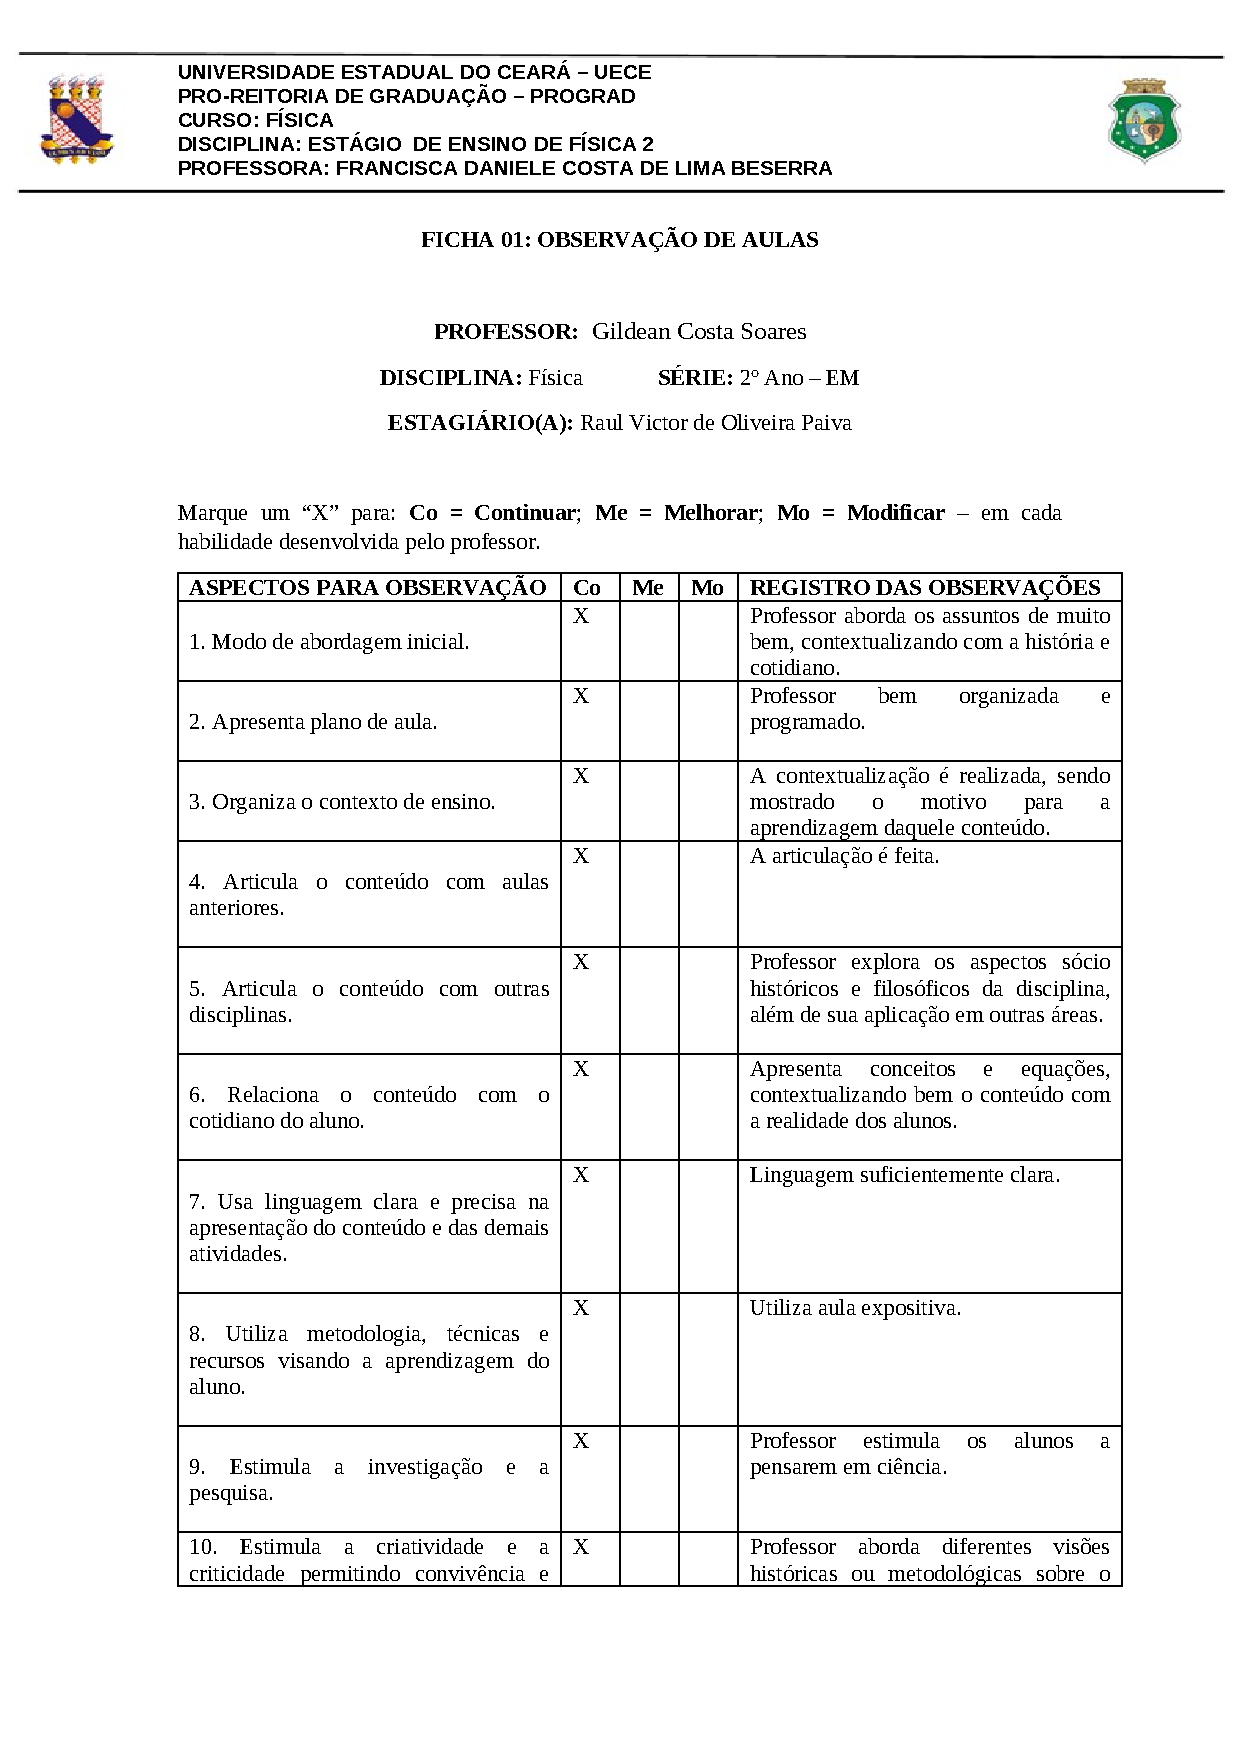
\includepdf[pages=-]{apendice/observacao} %% PARA INCLUIR BASTA RETIRAR A PORCETAGEM ANTES DE "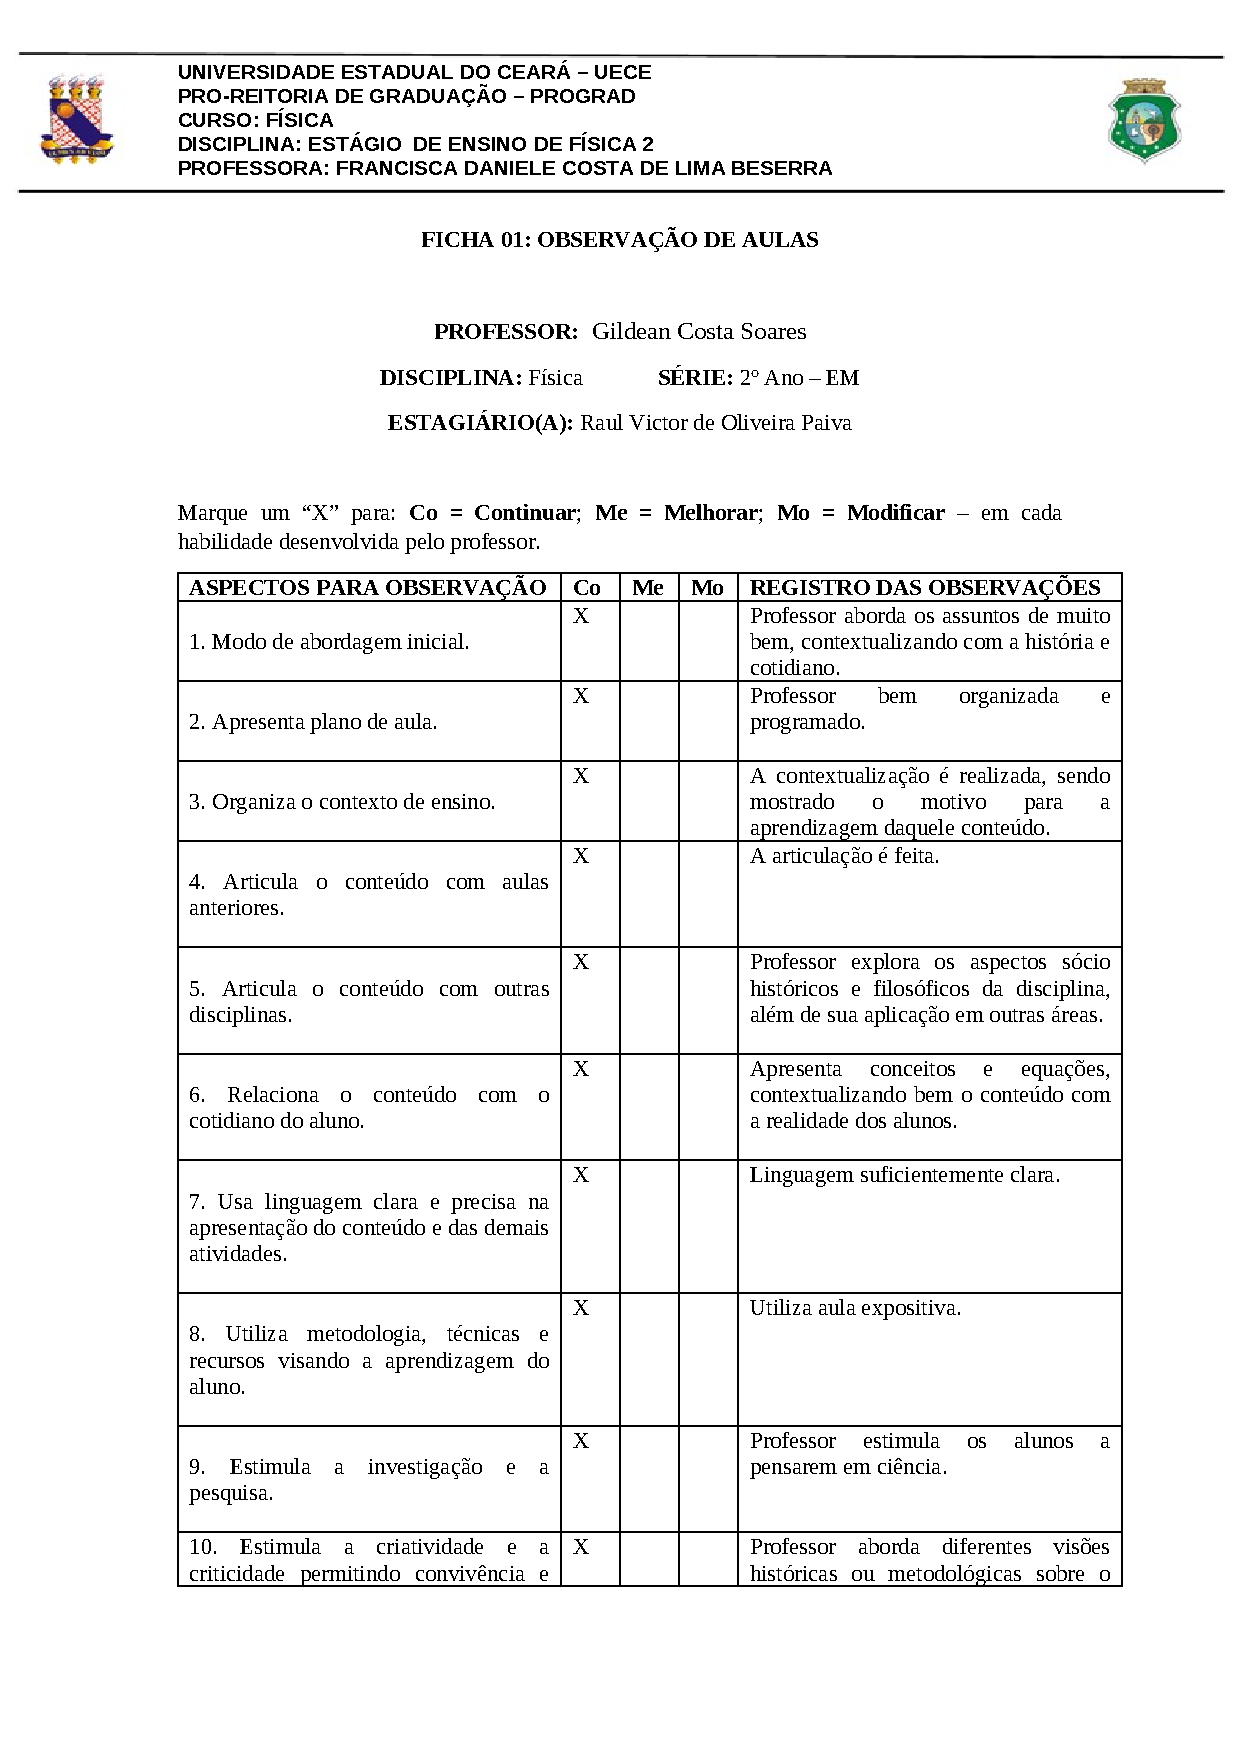
\includepdf[pages=-]{apendice/observacao}"
	


	%%% IMPORTANTE EXPORTAR O ARQUIVO DO PLANO DE AULA EM 'DOC' PARA PDF E SER PUXADO AQUI %%%
	\section{Plano de aula 1}
	\label{ap:plano1}  
	%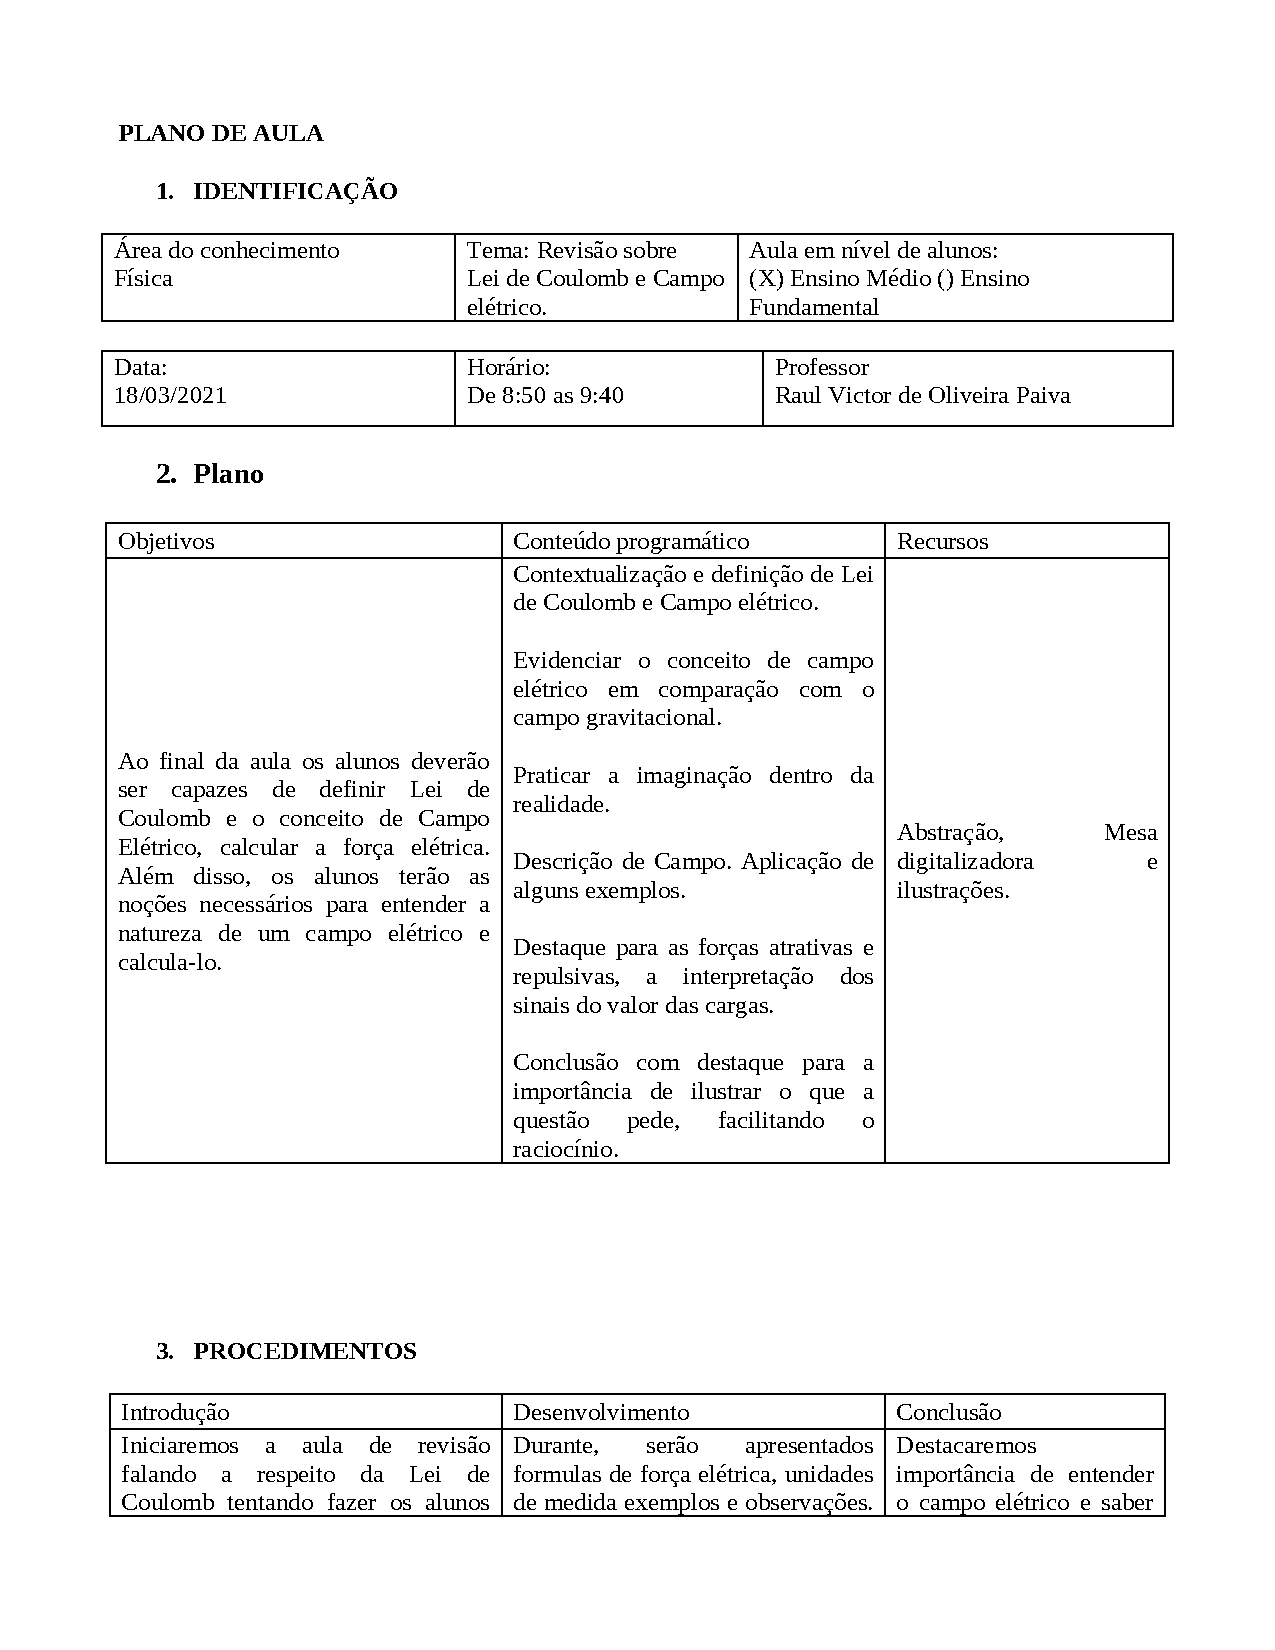
\includepdf[pages=-]{apendice/PLANO_DE_AULA_1}    %% PARA INCLUIR BASTA RETIRAR A PORCETAGEM ANTES DE "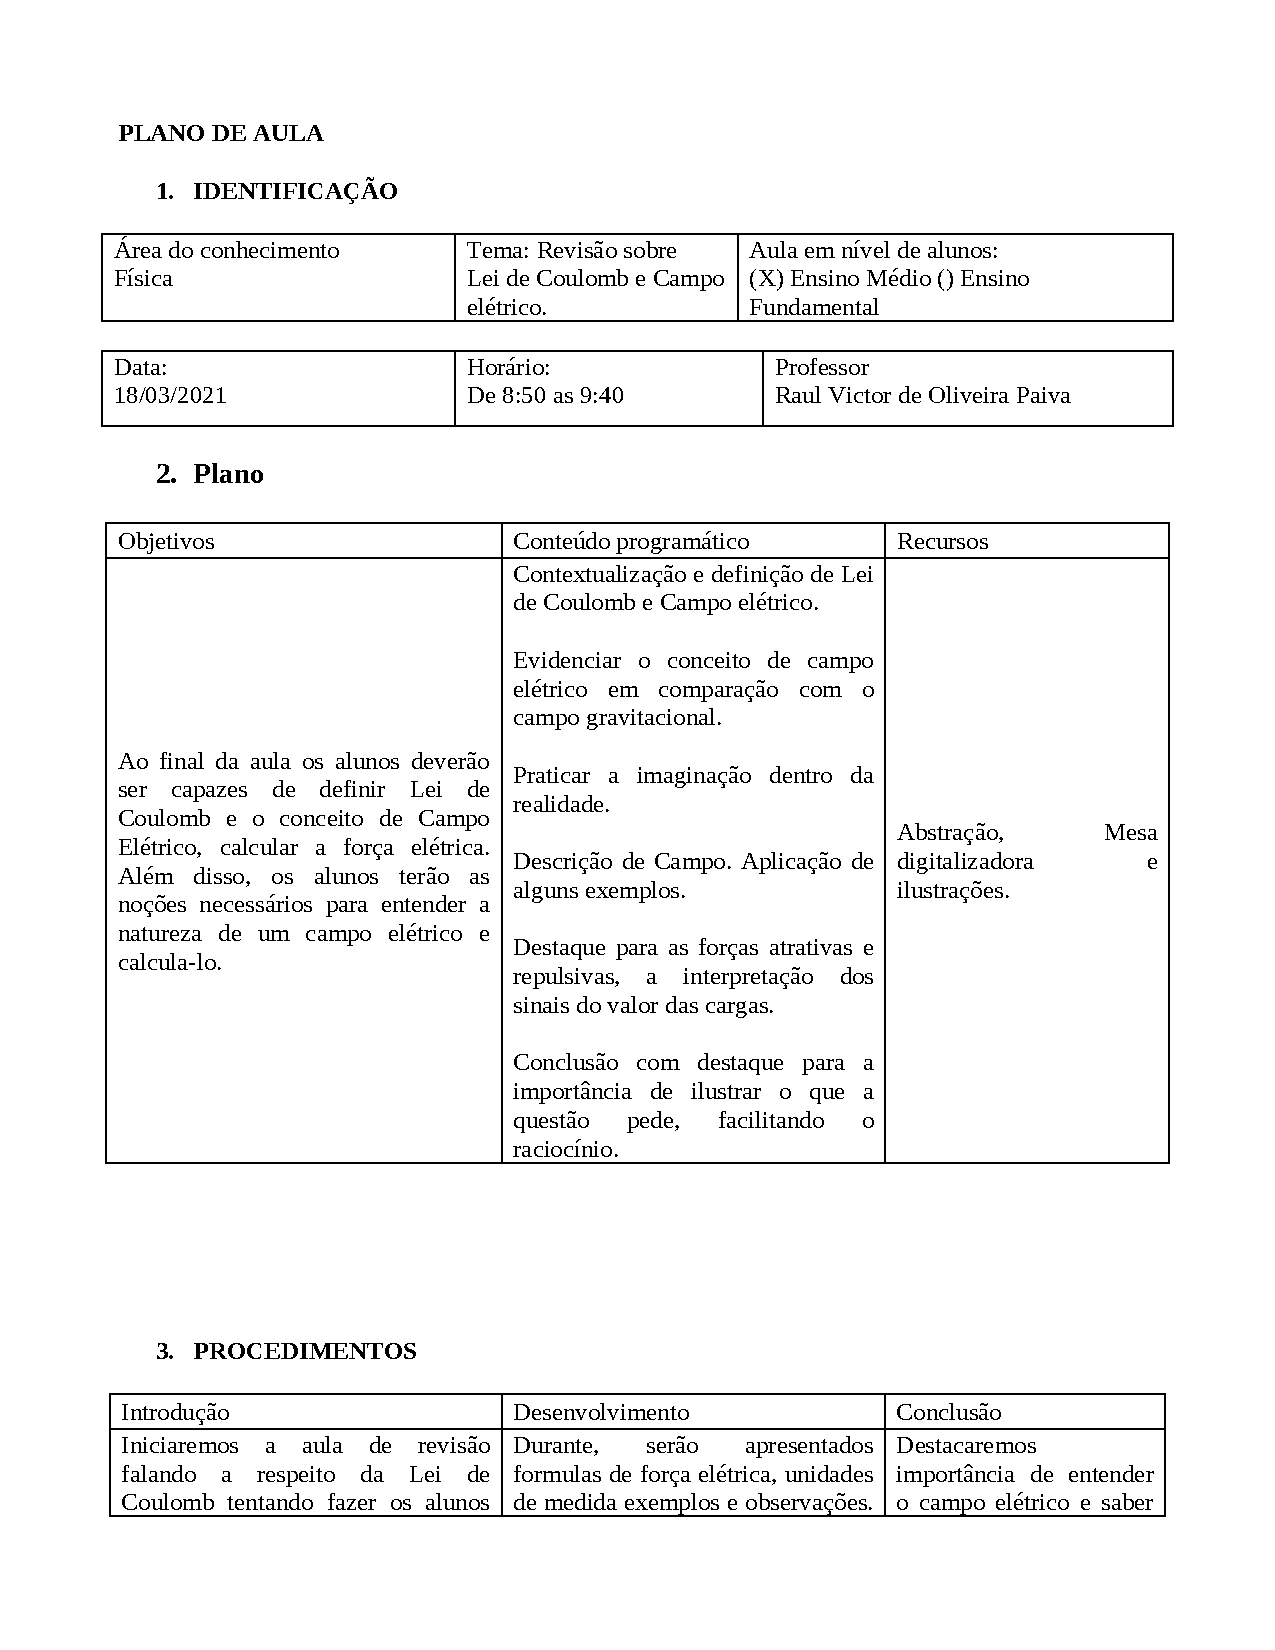
\includepdf[pages=-]{apendice/PLANO_DE_AULA_1}"
	
\end{document}